\documentclass[10pt,a4paper,titlepage]{report}
\usepackage[utf8]{inputenc}
\usepackage{amsmath}
\usepackage{amsfonts}
\usepackage{amssymb}
\usepackage{graphicx}
\usepackage{xcolor}
\usepackage{minted}

\begin{document}
\begin{titlepage}
\author{Rwithik Manoj}
\title{Shell Scripting\\Set 1}
\date{\today}
\maketitle
\end{titlepage}
\nonstopmode
\begin{enumerate}
\item Write a shell script to show various system configuration like
\begin{enumerate}
\item Currently logged user and his login name
\item Your current shell
\item Your home directory
\item Your operating system type
\item Your current path setting
\item Your current working directory
\item Number of users currently logged in
\end{enumerate}
\textbf{Script:}\newline
\inputminted{bash}{../Scripts/Expt4.sh}
\textbf{Output:}\newline 
\newline
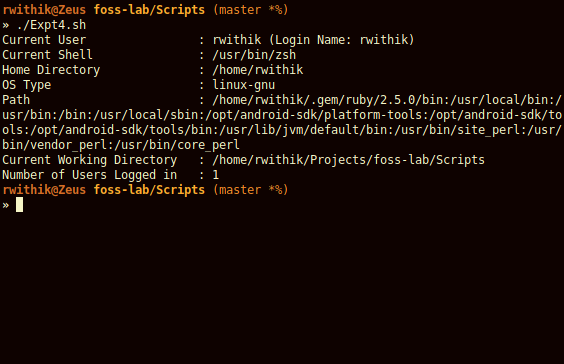
\includegraphics[width=\linewidth]{../Images/Shell1/1.png}
\pagebreak
\item Write a shell script to show various system configurations like
\begin{itemize}
\item Your OS and version, release number, kernel version
\item All available shells
\item Computer CPU information like processor type, speed etc
\item Memory information
\item Hard disk information like size of hard-disk, cache memory, model etc
\item File system (Mounted)
\end{itemize}
\textbf{Script:}\newline
\inputminted{bash}{../Scripts/Expt5.sh}
\textbf{Output:}\newline
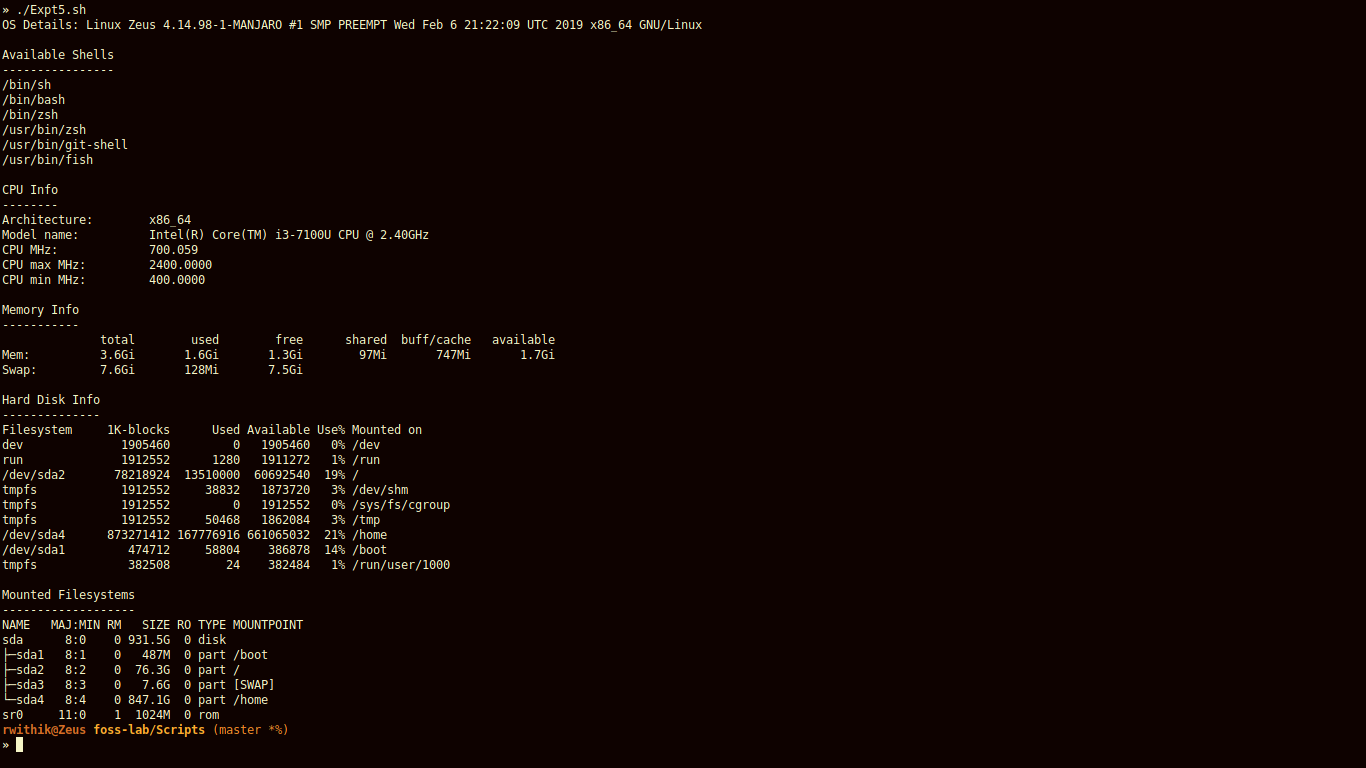
\includegraphics[width=\linewidth]{../Images/Shell1/2.png}
\item Write a shell script to implement a menu driven calculator with following functions
\begin{enumerate}
\item Addition
\item Subtraction
\item Multiplication
\item Division
\item Modulus
\end{enumerate}
\textbf{Script:}\newline
\inputminted{bash}{../Scripts/Expt6.sh}
\textbf{Output:}\newline
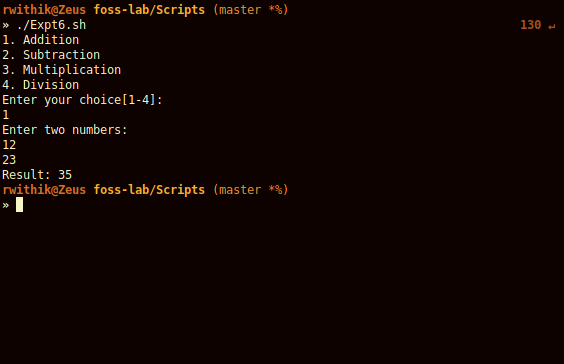
\includegraphics[width=\linewidth]{../Images/Shell1/3.png}
\pagebreak
\item Write a script called addnames that is to be called as follows ./addnames ulist username. Here ulist is the name of the file that contains list of user names and username is a particular student's username. The script should
\begin{enumerate}
\item Check that the correct number of arguments was received and print a message, in case the	number of arguments is incorrect
\item Check whether the ulist file exists and print an error message if it does not
\item Check whether the username already exists in the file. If the username exists, print a message stating that the name already exists. Otherwise, add the username to the end of the list.
\end{enumerate}
\textbf{Script:}\newline
\inputminted{bash}{../Scripts/Expt7.sh}
\textbf{Output:}\newline
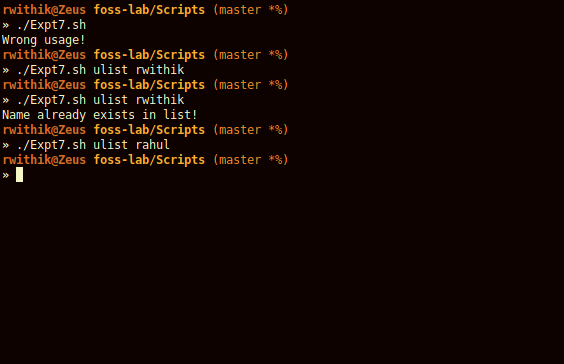
\includegraphics[width=\linewidth]{../Images/Shell1/4.png}
\pagebreak
\item Write a Shell script which starts on system boot up and kills every process which uses more than a specified amount of memory or CPU.\newline
\textbf{Script:}\newline
\inputminted{bash}{../Scripts/Expt8.sh}
\textbf{Output:}\newline
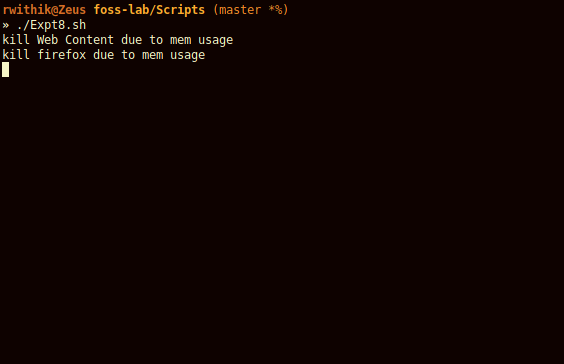
\includegraphics[width=\linewidth]{../Images/Shell1/5.png}
\end{enumerate}

\end{document}
